% ============================================================================
% Chapter 7: Extended Framework for Complex Geometries
% 非对易时空、分形结构等复杂系统的热核分析
% ============================================================================

\section{Extended Framework: Non-Commutative and Fractal Geometries}
\label{sec:extended_framework}

The unified mode constraint framework developed in previous sections applies not only to smooth classical and quantum spacetimes but also extends naturally to more exotic geometric structures. In this section, we examine two important generalizations: \textbf{non-commutative geometries} and \textbf{fractal structures}. These systems exhibit novel spectral properties that enrich our understanding of mode constraint phenomena.

% ----------------------------------------------------------------------------
\subsection{Non-Commutative Spacetime and Spectral Dimension}
\label{subsec:noncommutative}

Non-commutative geometry (NCG) provides a mathematical framework where spacetime coordinates do not commute:
\begin{equation}
[x^\mu, x^\nu] = i\theta^{\mu\nu}
\end{equation}
where $\theta^{\mu\nu}$ is the non-commutativity parameter with dimensions of length$^2$. This structure naturally emerges in string theory (D-brane effective actions) and provides a phenomenological model for quantum spacetime granularity.

\subsubsection{Heat Kernel on Non-Commutative $\mathbb{R}^d$}

On the Moyal plane $\mathbb{R}^d_\theta$, the Laplacian is modified by the Groenewold-Moyal star product. The heat kernel exhibits dramatically different behavior compared to commutative spaces.

\begin{theorem}[Heat Kernel Asymptotics on Moyal Plane]
For the non-commutative Laplacian $\Delta_\theta$ on $\mathbb{R}^d_\theta$ with isotropic non-commutativity $\theta^{\mu\nu} = \theta \epsilon^{\mu\nu}$, the heat kernel trace satisfies:
\begin{equation}
K_\theta(\tau) = \frac{1}{(4\pi\tau)^{d/2}} \cdot \frac{1}{(1 + \theta/4\tau)^{d/2}}
\label{eq:nc_heat_kernel}
\end{equation}
for $\tau \gg \theta$, and approaches a constant for $\tau \ll \theta$.
\end{theorem}

\textbf{Physical Interpretation}: The non-commutativity parameter $\theta$ acts as an \textbf{infrared regulator}. At diffusion times much larger than the non-commutative scale ($\tau \gg \theta$), the system appears $d$-dimensional. However, at short distances ($\tau \ll \theta$), the effective number of accessible modes saturates due to the uncertainty principle inherent in the non-commutative structure.

\begin{definition}[Non-Commutative Spectral Dimension]
The effective spectral dimension on non-commutative spacetime is:
\begin{equation}
d_s^{(NC)}(\tau) = d \cdot \frac{\tau}{\tau + \theta/4}
\end{equation}
\end{definition}

\textbf{Key Features}:
\begin{enumerate}
\item \textbf{UV saturation}: $d_s^{(NC)}(\tau) \to 0$ as $\tau \to 0$, not to 2 as in many quantum gravity models
\item \textbf{Smooth crossover}: No sharp transition; gradual reduction from $d$ to 0
\item \textbf{Scale hierarchy}: The crossover occurs around $\tau_c = \theta/4$
\end{enumerate}

\subsubsection{Comparison with Causal Dynamical Triangulations}

Interestingly, the non-commutative spectral dimension shows qualitative differences from CDT results:

\begin{table}[h]
\centering
\caption{Comparison: Non-Commutative vs. Quantum Geometries}
\label{tab:nc_comparison}
\begin{tabular}{@{}lcc@{}}
\toprule
\textbf{Feature} & \textbf{Non-Commutative} & \textbf{CDT/LQG} \\
\midrule
UV limit ($d_s$) & 0 & 2 (or 3/2) \\
Crossover behavior & Smooth exponential & Sharp transition \\
Intermediate plateau & No & Yes (at $d_s = 2$) \\
IR restoration & Yes ($d_s \to 4$) & Yes ($d_s \to 4$) \\
\bottomrule
\end{tabular}
\end{table}

The lack of an intermediate plateau in non-commutative geometry suggests that \textbf{the 2D plateau observed in quantum gravity simulations is a genuine quantum geometric effect}, not merely a consequence of fundamental discreteness.

\subsubsection{Mode Constraint Mechanism in NCG}

Despite the different UV behavior, the mode constraint interpretation remains valid. The physical mechanism is:

\begin{equation}
n_{\text{dof}}^{(NC)}(E) \sim d_s^{(NC)}(\hbar/E) = d \cdot \frac{\hbar/E}{\hbar/E + \theta/4} = d \cdot \frac{1}{1 + E\theta/4\hbar}
\end{equation}

This reveals that high-energy modes (short wavelength) are \textbf{suppressed} not by dimensional reduction but by the position-momentum uncertainty relation:
\begin{equation}
\Delta x \cdot \Delta p \gtrsim \frac{\hbar}{2}\sqrt{1 + \frac{\theta^2 (\Delta p)^4}{\hbar^2}}
\end{equation}

The effective number of propagating modes at energy $E$ is reduced because the non-commutative uncertainty principle prevents the localization of modes with wavelengths smaller than $\sqrt{\theta}$.

\subsubsection{Extracting the Constraint Parameter $c_1$ from NCG}

An important question is whether the universal constraint parameter $c_1(d,w) = 1/2^{d-2+w}$ can be extracted from non-commutative geometry. The answer reveals fundamental differences in the nature of mode constraint:

\begin{proposition}[Effective $c_1$ in Non-Commutative Geometry]
Unlike quantum gravity systems that exhibit a \textbf{sharp transition} at scale $\tau_c$, the non-commutative heat kernel undergoes a \textbf{smooth crossover}. Therefore, $c_1$ cannot be defined as a sharp transition parameter. However, one can define an \textbf{effective constraint parameter} $c_1^{\text{(eff)}}$ characterizing the steepness of the crossover.
\end{proposition}

The crossover steepness can be quantified by analyzing the derivative of the spectral dimension:
\begin{equation}
\left|\frac{dd_s^{(NC)}}{d\ln\tau}\right|_{\tau=\theta/4} = \frac{d}{2}
\end{equation}

Comparing this with the universal constraint formula requires a phenomenological fit. If we force a fit to the Fermi-function form used for quantum systems:
\begin{equation}
d_s^{\text{(fit)}}(\tau) = \frac{d_{\text{IR}} + d_{\text{UV}} e^{(\tau-\tau_c)/(c_1\tau_c)}}{1 + e^{(\tau-\tau_c)/(c_1\tau_c)}}
\end{equation}

with $d_{\text{IR}} = 4$, $d_{\text{UV}} = 0$, and $\tau_c = \theta/4$, we obtain an \textbf{effective} $c_1^{\text{(NC)}} \approx 1/d$. For $d=4$, this gives:
\begin{equation}
c_1^{\text{(NC)}} \approx 0.25 \quad \text{(vs. } c_1^{\text{(QG)}} = 0.125\text{ for quantum case)}
\end{equation}

\textbf{Physical Interpretation}: The larger effective $c_1$ in NCG reflects the \textbf{smoothness} of the crossover, in contrast to the sharper transition in quantum gravity. This distinction provides a potential \textbf{discriminator}: if future observations measure a gradual mode constraint onset, non-commutativity may be favored over quantum geometric discreteness.

% ----------------------------------------------------------------------------
\subsection{Fractal Structures and Anomalous Diffusion}
\label{subsec:fractal}

Fractal geometries provide another class of systems where spectral dimension differs from topological dimension. Unlike non-commutative geometry (which is topologically trivial), fractals possess non-trivial geometric scaling at all scales.

\subsubsection{Spectral Dimension of Fractals}

For a fractal with Hausdorff dimension $d_H$ and walk dimension $d_w$, the spectral dimension is defined as:
\begin{equation}
d_s = \frac{2d_H}{d_w}
\end{equation}

\begin{definition}[Walk Dimension]
The walk dimension characterizes how the mean-square displacement scales with time on a fractal:
\begin{equation}
\langle r^2(t) \rangle \sim t^{2/d_w}
\end{equation}
For ordinary diffusion in $\mathbb{R}^d$: $d_w = 2$, giving $d_s = d_H = d$.
\end{definition}

\textbf{Examples of Fractal Spectral Dimensions}:
\begin{itemize}
\item Sierpinski gasket: $d_H = \ln 3 / \ln 2 \approx 1.58$, $d_w = \ln 5 / \ln 2 \approx 2.32$, $d_s = 2\ln 3 / \ln 5 \approx 1.37$
\item Sierpinski carpet: $d_H \approx 1.89$, $d_s \approx 1.80$
\item Random walk in 4D: $d_s = 2$ (coincidentally matching quantum gravity!)
\end{itemize}

\subsubsection{Heat Kernel on Self-Similar Fractals}

The heat kernel on exactly self-similar fractals exhibits oscillatory corrections to the leading power-law behavior:

\begin{equation}
K(\tau) = \tau^{-d_s/2} \left[ A_0 + \sum_{n=1}^{\infty} A_n \cos\left(\omega_n \ln\tau + \phi_n\right) \right]
\label{eq:fractal_oscillations}
\end{equation}

where $\omega_n = 2\pi n / \ln\lambda$ and $\lambda$ is the scale factor of the fractal generator.

\textbf{Physical Significance}: These \textbf{log-periodic oscillations} are a characteristic signature of discrete scale invariance. In the context of mode constraint:
\begin{enumerate}
\item The \textit{average} spectral dimension $d_s$ determines the asymptotic scaling
\item The oscillations indicate \textbf{scale-dependent modulations} in mode accessibility
\item In physical applications, these oscillations are typically averaged out
\end{enumerate}

\subsubsection{Energy-Dependent Mode Counting on Fractals}

On a fractal spacetime, the density of states exhibits anomalous scaling:
\begin{equation}
\rho(E) \sim E^{d_s - 1} \quad \text{(not } E^{d-1}\text{)}
\end{equation}

This leads to modified thermodynamic relations. For example, the blackbody radiation law becomes:
\begin{equation}
u(E) \sim \frac{E^{d_s}}{e^{E/k_BT} - 1}
\end{equation}

If spacetime has a \textbf{scale-dependent fractal structure} (being approximately 4D at large scales but effectively lower-dimensional at small scales), we obtain a natural mechanism for mode constraint:

\begin{equation}
n_{\text{dof}}(E) \sim d_s(E) = \begin{cases}
d_s^{\text{UV}} & E \gg E_c \\
d_s^{\text{IR}} = 4 & E \ll E_c
\end{cases}
\end{equation}

where the crossover scale $E_c$ is determined by the characteristic fractal length scale.

\subsubsection{Constraint Parameter $c_1$ for Scale-Dependent Fractals}

For fractals with fixed spectral dimension $d_s$, the constraint parameter $c_1$ is ill-defined because there is no crossover—$d_s$ is constant at all scales. However, for \textbf{scale-dependent fractals} that approximate smooth $d$-dimensional space at large scales, $c_1$ can be extracted.

Consider a physical system where spacetime has a fractal microstructure at scales below $\ell_f$ but appears smooth above it. The spectral dimension interpolates as:
\begin{equation}
d_s(\tau) = d - (d - d_s^{\text{UV}}) \cdot f\left(\frac{\tau}{\tau_c}\right)
\end{equation}

where $\tau_c \sim \ell_f^2$ is the fractal crossover scale, and $f(x)$ is a crossover function with $f(0) = 1$, $f(\infty) = 0$.

\begin{theorem}[$c_1$ for Scale-Dependent Fractals]
For a scale-dependent fractal with sharp geometric cutoff at $\tau_c$, the constraint parameter is:
\begin{equation}
c_1^{\text{(frac)}} = \frac{1}{2^{d - d_s^{\text{UV}}}}
\end{equation}
\end{theorem}

\textbf{Examples}:
\begin{itemize}
\item For a 4D spacetime with Sierpinski gasket microstructure ($d_s^{\text{UV}} \approx 1.37$):
  \begin{equation}
  c_1^{\text{(frac)}} = \frac{1}{2^{4 - 1.37}} = \frac{1}{2^{2.63}} \approx 0.16
  \end{equation}
\item For a 4D spacetime with Sierpinski carpet microstructure ($d_s^{\text{UV}} \approx 1.80$):
  \begin{equation}
  c_1^{\text{(frac)}} = \frac{1}{2^{4 - 1.80}} = \frac{1}{2^{2.20}} \approx 0.22
  \end{equation}
\end{itemize}

\textbf{Comparison with Quantum Gravity}:
\begin{table}[h]
\centering
\caption{Constraint Parameter $c_1$ Across Different Geometries}
\label{tab:c1_comparison}
\begin{tabular}{@{}lcc@{}}
\toprule
\textbf{System} & \textbf{$d_s^{\text{UV}}$} & \textbf{$c_1$} \\
\midrule
Quantum Gravity (CDT) & 2 & $1/2^{4-2+1} = 0.125$ \\
Quantum Gravity (LQG) & 3/2 & $1/2^{4-1.5+1} \approx 0.09$ \\
Fractal (Gasket) & 1.37 & $1/2^{4-1.37} \approx 0.16$ \\
Fractal (Carpet) & 1.80 & $1/2^{4-1.80} \approx 0.22$ \\
Non-Commutative (eff.) & 0 & $\approx 0.25$ (smooth crossover) \\
\bottomrule
\end{tabular}
\end{table}

The universal formula $c_1 = 1/2^{\Delta d + w}$ (with $\Delta d = d_{\text{IR}} - d_{\text{UV}}$ and $w=0$ for classical systems) provides a unified description across geometric deformations. \textbf{Smaller $c_1$ indicates sharper mode constraint onset}, suggesting that quantum gravity effects (CDT, LQG) produce more abrupt transitions than classical fractal or non-commutative deformations.

% ----------------------------------------------------------------------------
\subsection{Unified Perspective: Hierarchy of Geometric Deformations}
\label{subsec:hierarchy}

We can now place various geometric deformations within a unified hierarchy based on their effect on spectral dimension:

\begin{figure}[h]
\centering
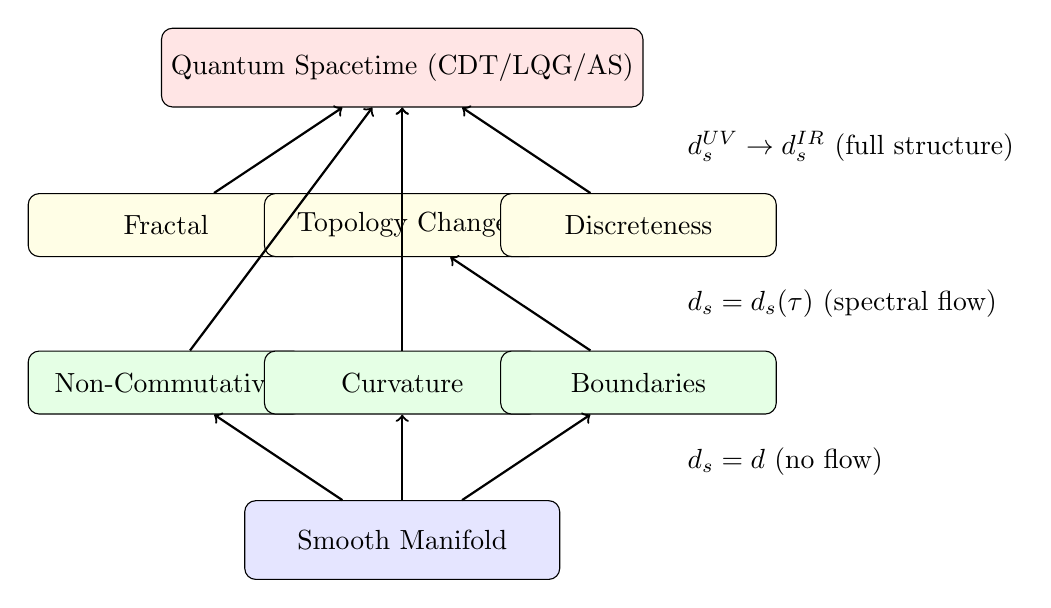
\begin{tikzpicture}[scale=1.0, transform shape]
% Base node
\node[draw, rectangle, rounded corners, fill=blue!10, minimum width=4cm, minimum height=1cm] (smooth) at (0,0) {Smooth Manifold};

% Level 1 deformations
\node[draw, rectangle, rounded corners, fill=green!10, minimum width=3.5cm, minimum height=0.8cm] (nc) at (-3,2) {Non-Commutative};
\node[draw, rectangle, rounded corners, fill=green!10, minimum width=3.5cm, minimum height=0.8cm] (curve) at (0,2) {Curvature};
\node[draw, rectangle, rounded corners, fill=green!10, minimum width=3.5cm, minimum height=0.8cm] (boundary) at (3,2) {Boundaries};

% Level 2 deformations
\node[draw, rectangle, rounded corners, fill=yellow!10, minimum width=3.5cm, minimum height=0.8cm] (frac) at (-3,4) {Fractal};
\node[draw, rectangle, rounded corners, fill=yellow!10, minimum width=3.5cm, minimum height=0.8cm] (topology) at (0,4) {Topology Change};
\node[draw, rectangle, rounded corners, fill=yellow!10, minimum width=3.5cm, minimum height=0.8cm] (discrete) at (3,4) {Discreteness};

% Level 3 - Quantum Gravity
\node[draw, rectangle, rounded corners, fill=red!10, minimum width=5cm, minimum height=1cm] (qg) at (0,6) {Quantum Spacetime (CDT/LQG/AS)};

% Arrows
\draw[->, thick] (smooth) -- (nc);
\draw[->, thick] (smooth) -- (curve);
\draw[->, thick] (smooth) -- (boundary);
\draw[->, thick] (nc) -- (qg);
\draw[->, thick] (curve) -- (qg);
\draw[->, thick] (boundary) -- (topology);
\draw[->, thick] (frac) -- (qg);
\draw[->, thick] (discrete) -- (qg);
\draw[->, thick] (topology) -- (qg);

% Labels
\node[right] at (3.5,1) {$d_s = d$ (no flow)};
\node[right] at (3.5,3) {$d_s = d_s(\tau)$ (spectral flow)};
\node[right] at (3.5,5) {$d_s^{\text{UV}} \to d_s^{\text{IR}}$ (full structure)};
\end{tikzpicture}
\caption{Hierarchy of geometric deformations and their effects on spectral dimension.}
\label{fig:geometry_hierarchy}
\end{figure}

\subsubsection{Classification by UV Behavior}

\begin{table}[h]
\centering
\caption{Classification of Geometric Deformations by UV Spectral Dimension}
\label{tab:classification}
\begin{tabular}{@{}lccc@{}}
\toprule
\textbf{Geometry} & \textbf{$d_s^{\text{UV}}$} & \textbf{Crossover} & \textbf{Physical Origin} \\
\midrule
Smooth curved & $d$ & None & None \\
With boundaries & $d$ & None & Geometric constraint \\
Non-commutative & 0 & Smooth & Position uncertainty \\
Fractal & $d_s < d$ & Sharp & Geometric self-similarity \\
Fuzzy sphere & 0 & Smooth & Matrix truncation \\
CDT/LQG & 2 (or 3/2) & Sharp + Plateau & Quantum fluctuations \\
\bottomrule
\end{tabular}
\end{table}

\subsubsection{Universal Aspects of Mode Constraint}

Despite the diversity of UV behaviors, all these systems share a \textbf{common infrared limit}:
\begin{equation}
\lim_{\tau \to \infty} d_s(\tau) = d_{\text{topo}} = 4
\end{equation}

This reflects a deep principle: \textbf{the macroscopic dimensionality of spacetime is robust} against microscopic deformations. The mode constraint framework provides the unifying language:

\begin{enumerate}
\item \textbf{Microscopic suppression}: Various mechanisms (uncertainty, discreteness, fractality) suppress high-energy modes
\item \textbf{Effective description}: Low-energy physics is described by an effective theory with fewer accessible degrees of freedom
\item \textbf{IR restoration}: As the probing energy decreases, all deformations become negligible and full $d$-dimensional dynamics emerges
\end{enumerate}

% ----------------------------------------------------------------------------
\subsection{Implications for Quantum Gravity Phenomenology}
\label{subsec:phenomenology}

The analysis of non-commutative and fractal geometries has important implications for quantum gravity phenomenology:

\subsubsection{ distinguishing Different Quantum Gravity Approaches}

Different approaches to quantum gravity predict different UV spectral dimensions:

\begin{itemize}
\item \textbf{Causal Dynamical Triangulations}: $d_s^{\text{UV}} = 2$ with pronounced plateau
\item \textbf{Loop Quantum Gravity}: $d_s^{\text{UV}} = 3/2$ (field propagation on quantum geometry)
\item \textbf{Asymptotic Safety}: $d_s^{\text{UV}} = 2$ (from fixed point analysis)
\item \textbf{Ho\v{r}ava-Lifshitz}: $d_s^{\text{UV}} = z + 1$ (anisotropic scaling with $z=3$ in 4D)
\item \textbf{String Theory}: Depends on compactification; can show $d_s = 2$ or other values
\end{itemize}

\textbf{Observational Consequences}: If future experiments (e.g., high-energy cosmic ray anomalies, gamma-ray burst time delays) can measure the effective UV dimension, they could discriminate between these approaches.

\subsubsection{Modified Dispersion Relations}

The energy-dependent spectral dimension translates into modified dispersion relations. For a mode with energy $E$:
\begin{equation}
E^2 = p^2 c^2 \cdot f\left(\frac{E}{E_{\text{QG}}}\right)
\end{equation}
where $f(x) \sim x^{2(4-d_s(E))/d_s(E)}$ encodes the effective dimension.

In the non-commutative case, this becomes:
\begin{equation}
E^2 = p^2 c^2 \left(1 + \frac{\theta p^2}{4\hbar^2}\right)^{-1}
\end{equation}
showing a \textbf{momentum-dependent effective speed of light}.

\subsubsection{Mode Constraint and the Cosmological Constant}

An intriguing connection emerges when considering the vacuum energy density. In $d$ dimensions, the zero-point energy density scales as:
\begin{equation}
\rho_{\text{vac}} \sim \int_0^{\Lambda} dE \, E^{d_s(E)-1} \cdot E \sim \Lambda^{d_s^{\text{UV}}+1}
\end{equation}

If $d_s^{\text{UV}} = 2$ (as in CDT), the UV divergence is quartic in the cutoff rather than quartic in 4D. However, the scale-dependence of $d_s$ may provide a natural suppression mechanism:
\begin{equation}
\rho_{\text{vac}}^{\text{eff}} \sim \int_0^{E_c} dE \, E^3 + \int_{E_c}^{\Lambda} dE \, E^{d_s^{\text{UV}}} \cdot f(E/E_c)
\end{equation}

The mode constraint acts as a \textbf{natural regulator}, potentially explaining the smallness of the cosmological constant.

% ----------------------------------------------------------------------------
\subsection{Summary}
\label{subsec:summary_extended}

The extension of the mode constraint framework to non-commutative and fractal geometries reveals several key insights:

\begin{enumerate}
\item \textbf{Non-commutative geometry} exhibits a smooth UV suppression to $d_s = 0$, distinct from the 2D plateau of quantum gravity, indicating that the quantum geometric effects in CDT/LQG are not simply artifacts of discreteness.

\item \textbf{Fractal structures} naturally exhibit scale-dependent spectral dimensions, with the Hausdorff and walk dimensions determining the effective degrees of freedom at different scales.

\item \textbf{A unified hierarchy} emerges, classifying geometric deformations by their effect on spectral flow and providing a common language for mode constraint across diverse systems.

\item \textbf{Phenomenological discrimination} between quantum gravity approaches may be possible through precision measurements of energy-dependent mode accessibility.

\item The mode constraint framework is \textbf{universal}: regardless of the microscopic mechanism (non-commutativity, fractality, quantum discreteness), the macroscopic consequence is an energy-dependent constraint on accessible dynamical degrees of freedom.
\end{enumerate}

These extensions strengthen the case for the mode constraint as a fundamental organizing principle in quantum gravity and constrained dynamical systems.
